%!TEX root = ../thesis-main.tex
\chapter{Tecnologie e Progettazione}
\label{chap:technologies}

Questo capitolo presenta l'analisi degli obiettivi e la progettazione del sistema EcoSpot, descrivendo l'architettura logica e le scelte tecnologiche adottate per lo sviluppo dell'applicazione mobile e la sua integrazione con i servizi cloud e IoT.

\section{Obiettivi del progetto}
\label{sec:project_goals}

La progettazione di EcoSpot è guidata da quattro obiettivi strategici, volti a coniugare l'esperienza turistica con la consapevolezza ecologica e le moderne tecnologie mobili.

\begin{itemize}
    \item \textbf{Divulgazione e Citizen Science:} l'obiettivo è diffondere la conoscenza della biodiversità locale attraverso una \textit{collezione digitale} strutturata e partecipativa. L'applicazione non si limita a offrire un catalogo dettagliato di specie (suddivise in categorie come uccelli, mammiferi, pesci e aree verdi), ma abilita pratiche di \textit{Citizen Science}: gli utenti possono contribuire attivamente al monitoraggio del territorio inviando segnalazioni georeferenziate e fotografiche, trasformando la semplice osservazione in un percorso di tutela condivisa.

    \item \textbf{Incentivazione del turismo lento:} il sistema mira a favorire un'esplorazione rispettosa del territorio sfruttando meccaniche \textit{location-based}. Grazie alla geolocalizzazione e al \textit{geofencing}, l'utente è incentivato a raggiungere fisicamente luoghi reali (valli, argini, punti di osservazione) per sbloccare i contenuti e validare le scoperte, promuovendo così una mobilità dolce e un presidio attivo degli habitat, in contrapposizione al turismo di massa.

    \item \textbf{Monitoraggio ambientale integrato:} il progetto intende rendere accessibili parametri ecologici complessi tramite l'aggregazione di dati IoT in tempo reale. L'app si interfaccia con le API di enti territoriali (es. progetto DISCOV.ER) per i dati idrografici (livello, temperatura, conducibilità) e integra servizi meteorologici come Open-Meteo \cite{open_meteo_api}, rendendo visibili all'utente fattori invisibili ma vitali per l'ecosistema lagunare.

    \item \textbf{Incremento del coinvolgimento (Gamification):} l'ultimo obiettivo è massimizzare la ritenzione e la partecipazione dell'utente attraverso la \textit{gamification}. L'uso di elementi ludici come punti esperienza (XP) e livelli dinamici (da ``Esploratore'' a ``Leggenda del Delta'') serve a rafforzare il senso di appartenenza al territorio e a stimolare comportamenti virtuosi, premiando l'interazione fisica con il Parco.
\end{itemize}

L'integrazione di questi quattro pilastri mira ad aumentare l'attenzione dei visitatori, offrendo un'esperienza che combina contenuti informativi, esplorazione fisica e feedback immediati sulle pratiche sostenibili. Al tempo stesso, la possibilità di accedere a dati ambientali in tempo quasi reale e di collegarli alle osservazioni sul campo contribuisce a sviluppare una maggiore consapevolezza ecologica, mostrando in modo concreto la fragilità e il valore degli ecosistemi lagunari. In questo senso, EcoSpot si configura non solo come strumento di guida turistica, ma come piattaforma di educazione ambientale e di supporto alla gestione sostenibile delle aree protette del Delta del Po.

\section{Tecnologie}
\label{sec:technologies}

\subsection{Flutter e Dart}
Per lo sviluppo dell'applicazione EcoSpot è stato selezionato \textbf{Flutter} \cite{flutter}, il framework open-source sviluppato da Google che consente la realizzazione di applicazioni multipiattaforma native.
Questa scelta architetturale è stata motivata da diversi fattori strategici che rispondono agli obiettivi del progetto:

\begin{itemize}
    \item \textbf{Efficienza nello sviluppo (Single Codebase):} Flutter permette di gestire un'unica base di codice per Android e iOS. Questo ha ridotto drasticamente i tempi di implementazione, garantendo al contempo una parità di funzionalità tra le piattaforme senza la necessità di mantenere due team di sviluppo distinti.

    \item \textbf{Prestazioni grafiche (Impeller):} A differenza di altri framework ibridi, Flutter non utilizza webview ma un motore di rendering proprietario. Per EcoSpot è stato sfruttato il moderno motore \textbf{Impeller}, che sostituisce il precedente Skia. Impeller risolve i problemi di \textit{jank} (scatti) dovuti alla compilazione degli shader a runtime, pre-compilandoli e sfruttando le API di basso livello (Metal su iOS e Vulkan su Android). Ciò garantisce animazioni fluide a 60 FPS, fondamentali per la gestione delle mappe interattive e delle transizioni nelle schede delle specie.

    \item \textbf{Produttività (Hot Reload):} La funzionalità di \textit{Stateful Hot Reload} ha permesso di visualizzare le modifiche al codice in tempo reale senza riavviare l'applicazione, accelerando il ciclo di test e il raffinamento dell'interfaccia utente (UI).

    \item \textbf{Ecosistema e Modularità:} La disponibilità di pacchetti maturi su \texttt{pub.dev} ha facilitato l'integrazione di funzionalità complesse. Librerie come \texttt{flutter\_map} per la cartografia, \texttt{geolocator} per il tracciamento GPS e \texttt{riverpod} per la gestione dello stato si sono rivelate essenziali per l'architettura del sistema.
\end{itemize}

Il linguaggio alla base del framework è \textbf{Dart}, scelto per la sua duplice natura: ottimizzato per la UI e fortemente orientato alla programmazione asincrona.
In particolare, il supporto nativo per \texttt{Future} e \texttt{Stream} si è rivelato cruciale per gestire i flussi di dati in tempo reale di EcoSpot, come l'aggiornamento della posizione dell'utente e il recupero dei dati dai sensori IoT, senza mai bloccare il thread principale dell'interfaccia.

Nel contesto del progetto, l'adozione di Flutter e Dart garantisce una soluzione scalabile e versatile, capace di sostenere i requisiti funzionali di gamification e citizen science offrendo un'esperienza utente di livello nativo.

\subsection{Backend, Servizi Cloud e API}
L'infrastruttura di backend costituisce il cuore della gestione dei dati e della persistenza delle informazioni, garantendo sincronizzazione in tempo reale, sicurezza e disponibilità del servizio. La scelta tecnologica è stata guidata da criteri di scalabilità, ridotta manutenzione infrastrutturale (approccio \textit{Serverless}) e facilità di integrazione con l'ecosistema mobile.

Le principali componenti progettuali includono:

\begin{itemize}
    \item \textbf{Architettura Serverless e Cloud Services:} A differenza delle architetture tradizionali, il sistema non utilizza un server monolitico proprietario ma si appoggia alla suite \textbf{Google Firebase} come Backend-as-a-Service (BaaS). Questo approccio delega la complessità della gestione server, permettendo all'applicazione di interagire direttamente con i servizi cloud tramite SDK nativi sicuri, garantendo alte prestazioni e riducendo i tempi di latenza.

    \item \textbf{Database NoSQL:} Il sistema utilizza \texttt{Cloud Firestore}, un database orientato ai documenti che consente all'app mobile di sincronizzare i dati in tempo reale tra i dispositivi. A differenza dei database relazionali, Firestore offre una struttura flessibile organizzata in collezioni (es. \texttt{users}, \texttt{reports}, \texttt{species}), ottimizzata per letture frequenti e funzionamento offline. La persistenza locale permette agli utenti di consultare i dati e salvare progressi anche in assenza di connettività, con sincronizzazione automatica al ripristino della rete.

    \item \textbf{Gestione della Logica e dello Stato (Controller):} La logica applicativa lato client e il flusso dei dati sono gestiti attraverso il framework \textbf{Riverpod}. I provider agiscono come controller intelligenti che orchestrano le operazioni asincrone: mediano le richieste tra l'interfaccia utente (UI) e i repository dei dati, aggiornando dinamicamente le viste senza bloccare il thread principale.

    \item \textbf{Autenticazione e Sicurezza:} Il modulo \texttt{Firebase Authentication} gestisce l'identità degli utenti, supportando un sistema ibrido che include l'accesso anonimo e l'autenticazione federata tramite terze parti (es. Google). Questo componente assicura che le operazioni di scrittura sul database (come l'invio di segnalazioni o l'aggiornamento dei livelli) siano consentite solo a utenti validati, proteggendo i dati sensibili attraverso regole di sicurezza lato server.

    \item \textbf{Elaborazione Gamification e Citizen Science:} Le attività di monitoraggio e le meccaniche di gioco sono processate attraverso una logica distribuita. Il client mobile calcola in tempo reale le interazioni spaziali (distanza dai POI tramite GPS), mentre il backend si occupa della validazione e dello storage delle segnalazioni fotografiche (\textit{Citizen Science}) tramite \texttt{Cloud Storage}, garantendo l'integrità del percorso di crescita dell'utente (XP e livelli).

    \item \textbf{Integrazione con API Esterne e IoT:} Il sistema è progettato per comunicare con servizi di terze parti per arricchire il contesto ambientale. L'applicazione consuma le API di \texttt{Open-Meteo} per i dati climatici e si interfaccia con endpoint dedicati per il recupero dei dati dai sensori \ac{IoT}, normalizzando formati eterogenei in un'unica esperienza utente coerente.
\end{itemize}

Questa architettura modulare consente di mantenere separati i livelli di presentazione (Widget Flutter), gestione dello stato (Riverpod) e servizi dati (Firebase/API), favorendo la manutenibilità del codice e la possibilità di estendere le funzionalità senza impattare sulla stabilità del sistema esistente.

\subsection{Gestione dello Stato: Riverpod}
La complessità derivante dalla gestione simultanea di flussi dati eterogenei è risolta mediante \textbf{Riverpod}. L'architettura dei provider orchestra i principali flussi applicativi distinguendo le sorgenti:
\begin{itemize}
    \item \textbf{Stream Providers:} Gestiscono i dati in tempo reale. Il \texttt{userPositionProvider} ascolta costantemente gli aggiornamenti del GPS, mentre \texttt{userProfileProvider} mantiene sincronizzata la UI con le modifiche al documento utente su Firestore.
    \item \textbf{Future Providers:} Gestiscono operazioni asincrone su richiesta singola. Il \texttt{speciesProvider} aggrega i dati statici delle specie con lo storico delle scoperte dell'utente per calcolare lo stato di sblocco, mentre \texttt{sensorsProvider} invoca i servizi esterni per il recupero dei dati telemetrici.
\end{itemize}

\subsection{Integrazione di Servizi e Fonti Dati}
Per raggiungere gli obiettivi di sensibilizzazione ambientale e gamification, EcoSpot non opera come un sistema isolato, ma agisce come collettore di dati provenienti da fonti eterogenee. L'architettura è stata progettata per integrare servizi di terze parti che arricchiscono l'esperienza utente con informazioni contestuali in tempo reale.
\begin{itemize}
    \item \textbf{Monitoraggio Ambientale e Consapevolezza}: l'integrazione con le reti di sensori IoT risponde all'esigenza educativa di rendere visibili parametri ecologici (come livello idrometrico e salinità) altrimenti invisibili al turista. La scelta di utilizzare dati reali serve a creare un collegamento diretto tra le condizioni chimico-fisiche dell'habitat e la biodiversità osservata, trasformando l'applicazione in uno strumento di divulgazione scientifica attiva.
    \item \textbf{Geolocalizzazione e Cartografia Open Source}: per la componente cartografica è stata scelta la piattaforma \textbf{OpenStreetMap}. Questa soluzione garantisce la flessibilità necessaria per rappresentare sentieri e aree naturali spesso assenti nelle mappe commerciali. L'approccio \textit{Location-Based} vincola l'accesso ai contenuti alla posizione fisica dell'utente, disincentivando la fruizione passiva e promuovendo l'esplorazione diretta del territorio.
    \item \textbf{Contestualizzazione Meteorologica}: le condizioni atmosferiche influenzano l'etologia delle specie e la fruibilità del parco. Il sistema integra servizi meteorologici esterni (come \textbf{Open-Meteo}) per fornire all'utente un quadro immediato delle condizioni ambientali. Questo dato non è puramente informativo, ma arricchisce le segnalazioni di \textit{Citizen Science}, permettendo di correlare gli avvistamenti faunistici con le variabili climatiche del momento.
\end{itemize}

\section{Architettura del Sistema}
\label{sec:system_architecture}

Dati i requisiti funzionali precedentemente definiti, è possibile delineare l'architettura logica del sistema EcoSpot. La struttura è concepita come un ecosistema modulare composto da quattro componenti principali, che collaborano per garantire un'esperienza utente reattiva e scalabile.

L'esperienza dell'utente è mediata interamente dallo \textit{smartphone}, che agisce sia come portale d'accesso ai contenuti sia come strumento di controllo delle funzionalità. L'applicazione integra \textbf{OpenStreetMap}, una piattaforma cartografica libera che fornisce dati geografici dettagliati e costantemente aggiornati da una comunità globale. 
A differenza delle soluzioni proprietarie, l'integrazione di OpenStreetMap (tramite il motore di rendering \texttt{flutter\_map}) consente una personalizzazione avanzata della visualizzazione dei sentieri e delle aree naturali del Delta, permettendo all'utente di orientarsi e navigare in tempo reale verso i punti di interesse (POI) disseminati nel territorio.

Il cuore della gestione dei dati è affidato a \textbf{Google Cloud Firestore}. Questo database NoSQL orientato ai documenti è utilizzato per memorizzare in modo strutturato tutte le informazioni vitali del sistema: dai profili utente ai progressi di gioco (livelli e XP), fino all'inventario delle specie scoperte (i dettagli sulla struttura dati sono approfonditi nella Sezione \ref{sec:data_modeling}). La scelta di utilizzare una soluzione cloud-based, supportata da \textbf{Cloud Storage} per l'archiviazione delle immagini fotografiche, risponde all'esigenza di centralizzare i contributi di \textit{Citizen Science}, rendendo le segnalazioni immediatamente sicure e accessibili per future analisi, garantendo al contempo la sincronizzazione dei dati tra diversi dispositivi dello stesso utente (si veda Sezione \ref{sec:citizen_science}).

Per la gestione delle logiche spaziali, il sistema sfrutta la potenza di calcolo locale del dispositivo attraverso il pacchetto \textbf{Geolocator}. Invece di dipendere costantemente dal server per ogni verifica, l'applicazione calcola direttamente sul client le distanze euclidee tra la posizione dell'utente e gli habitat. Questo approccio decentralizzato permette di validare le scoperte (meccanismo di \textit{geofencing}) in tempo reale e con latenza zero, riducendo il consumo di dati mobili e migliorando l'esperienza anche in aree con scarsa copertura di rete.

Infine, per contestualizzare l'esperienza nell'ambiente reale, il sistema agisce come un aggregatore di dati esterni tramite protocolli \textbf{HTTP/REST}. L'applicazione interroga periodicamente le API di servizi terzi, come le stazioni di monitoraggio IoT per i livelli idrometrici e il servizio \textbf{Open-Meteo} per le condizioni atmosferiche. Questa integrazione assicura che le informazioni mostrate all'utente non siano solo statiche, ma riflettano le condizioni dinamiche e vitali dell'ecosistema lagunare al momento della visita.

\begin{figure}[htbp]
    \centering
    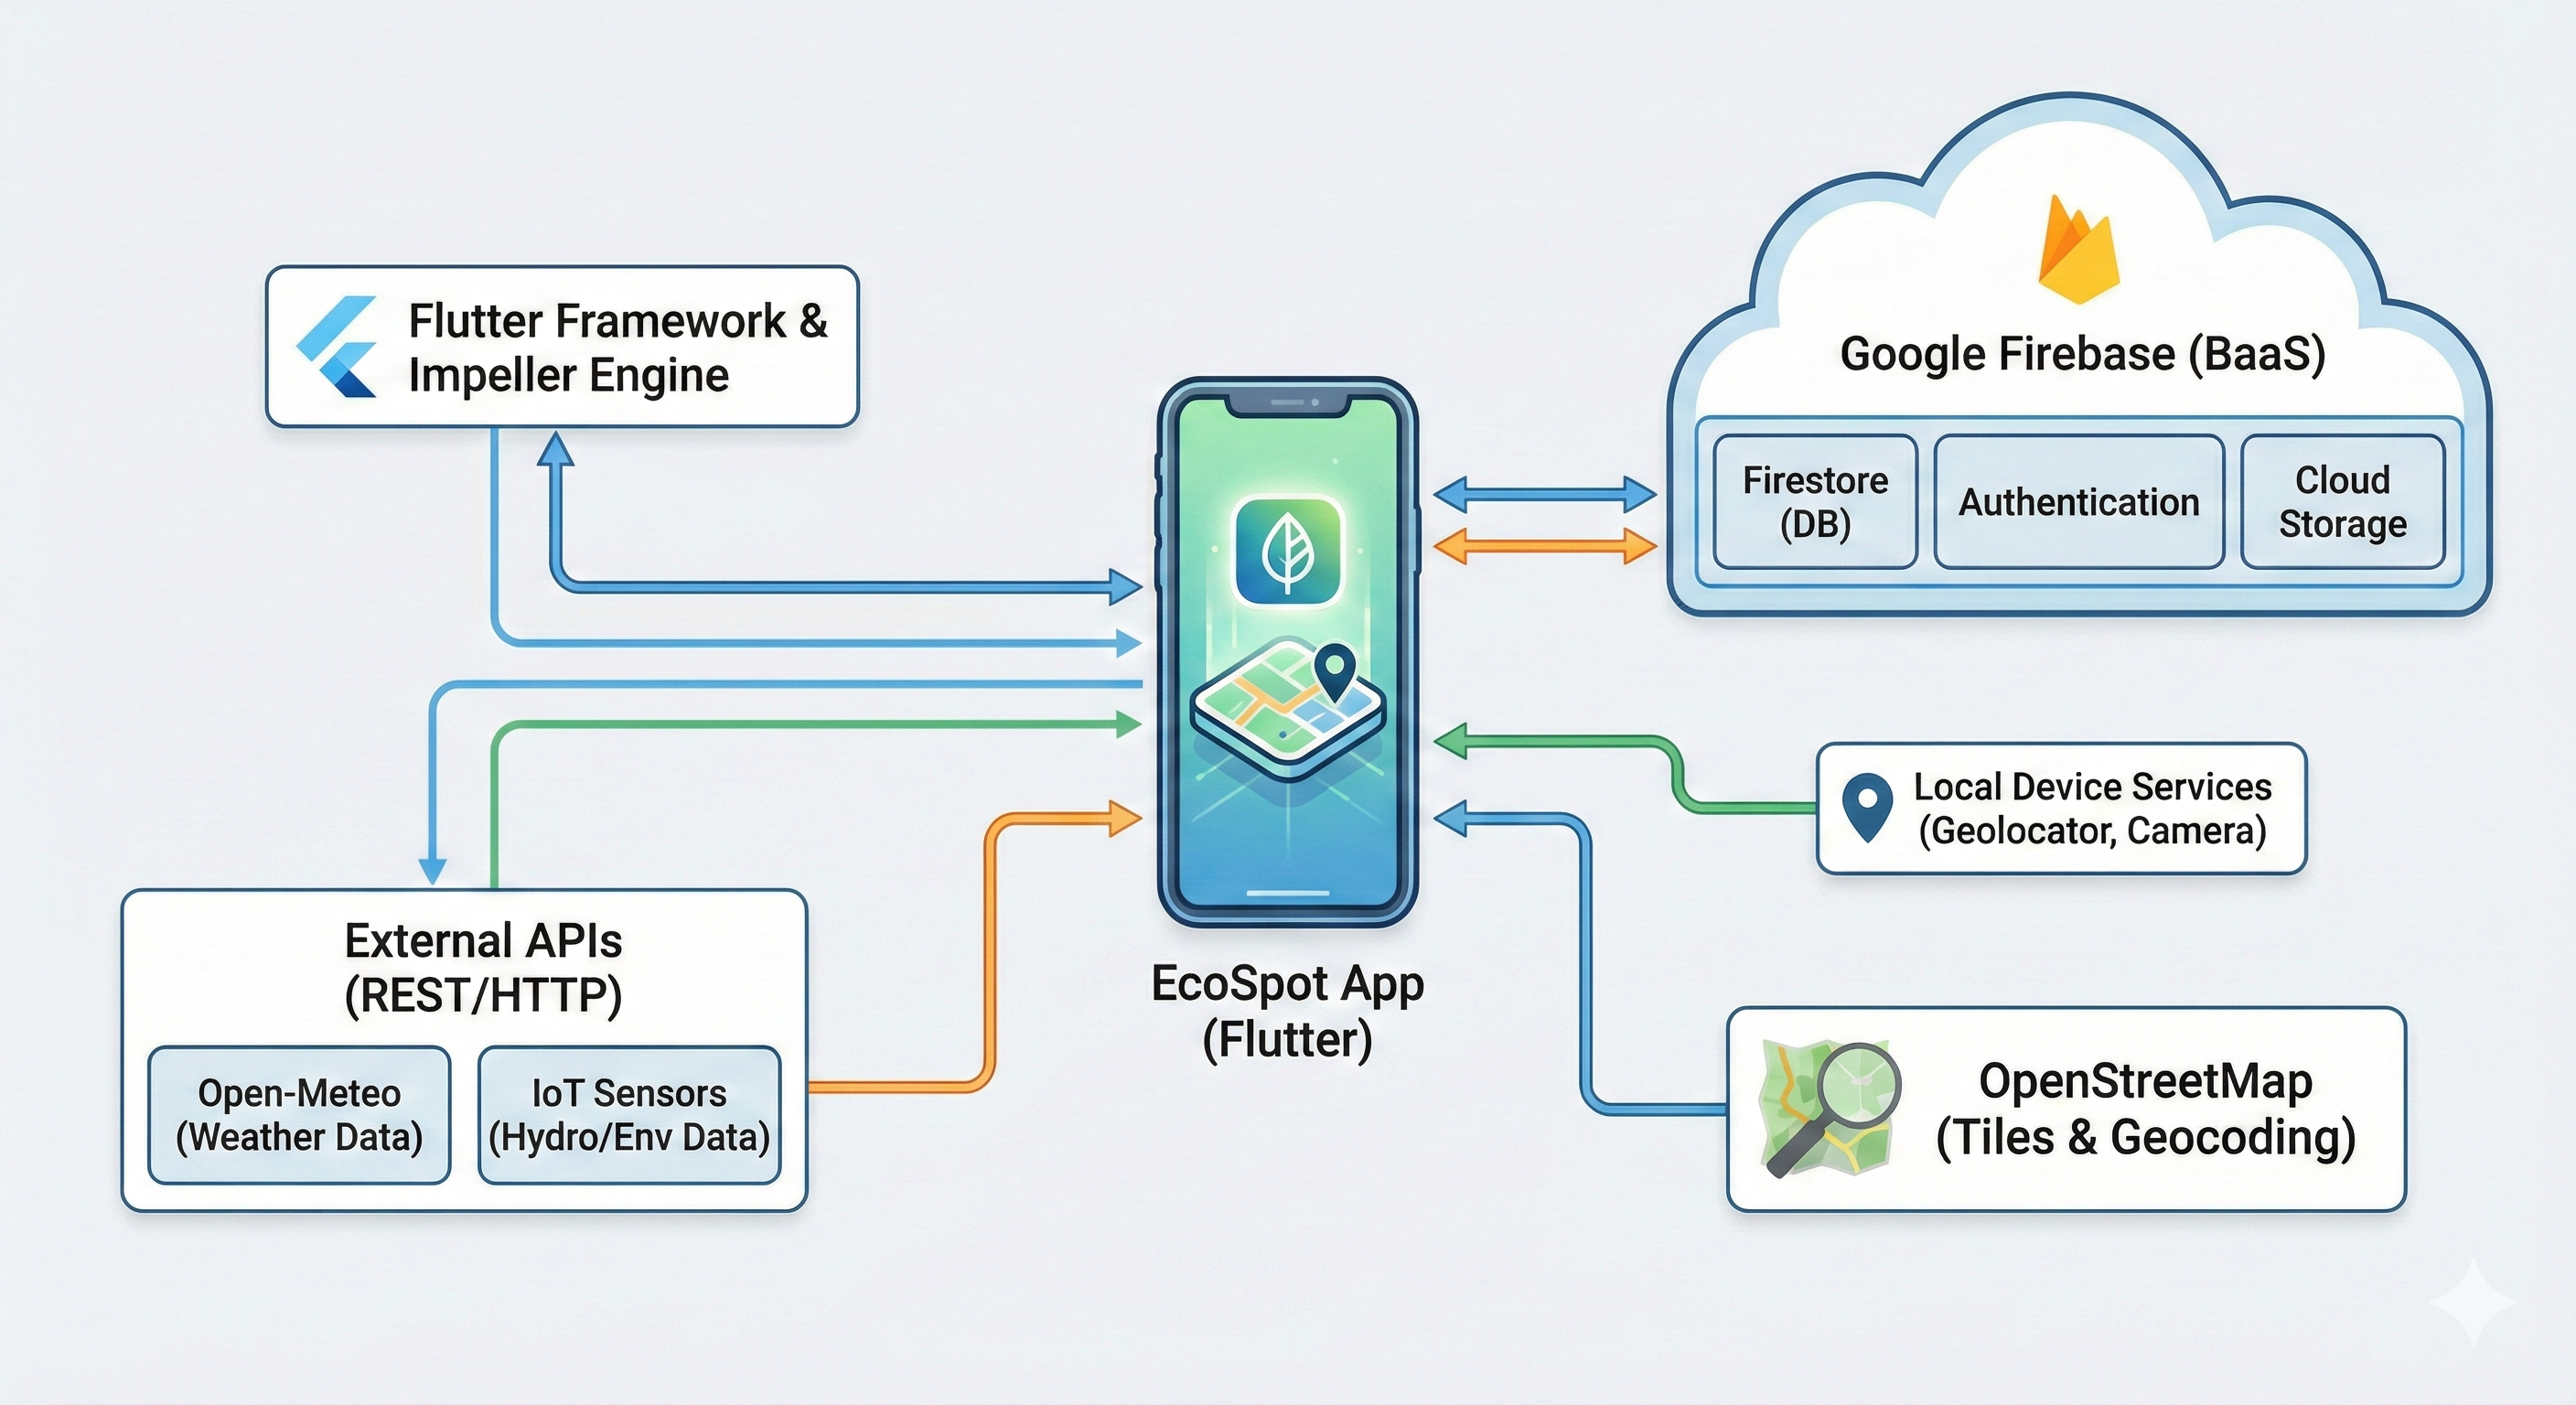
\includegraphics[width=0.9\textwidth]{figures/schema/architecture_schema.png}
    
    \caption[Schema Architetturale di EcoSpot]{Schema logico dell'architettura di sistema.}
    
    \label{fig:system_architecture_schema}
\end{figure}

\section{Modellazione e Gestione dei Dati}
\label{sec:data_modeling}

La modellazione dei dati rappresenta una fase cruciale della progettazione del sistema EcoSpot. A differenza dei sistemi tradizionali basati su schemi rigidi relazionali, l'adozione di un'architettura \textbf{NoSQL Document-Oriented} (tramite Google Cloud Firestore) ha richiesto un approccio orientato alla flessibilità, alla scalabilità orizzontale e all'ottimizzazione delle performance di lettura. 

Questa sezione analizza i requisiti informativi che hanno guidato la progettazione e descrive in dettaglio le entità logiche e le loro relazioni, garantendo che il sistema supporti efficacemente le funzionalità di gamification, citizen science e monitoraggio ambientale.

\subsection{Requisiti Informativi del Sistema}
Durante la fase di analisi dei requisiti, sono state identificate le necessità informative fondamentali che la base di dati deve soddisfare per abilitare le funzionalità dell'applicazione EcoSpot. La struttura dati è stata modellata per rispondere alle seguenti esigenze operative:

\begin{itemize}
    \item \textbf{Utente:} Il sistema deve mantenere un profilo utente persistente e sincronizzato tra i dispositivi. Oltre ai dati anagrafici di base (gestiti tramite provider di autenticazione), il database deve memorizzare in tempo reale lo stato di avanzamento nel gioco, includendo il livello raggiunto, i punti esperienza (XP) accumulati e l'inventario delle specie già scoperte.
    
    \item \textbf{Interazione Location-Based:} Per supportare la meccanica del ``Turismo Lento'', il modello dati deve associare ogni entità biologica o punto di interesse a coordinate geografiche precise (latitudine e longitudine) e a soglie di tolleranza specifiche (raggio di scoperta). Il sistema deve permettere query spaziali efficienti o verifiche lato client per determinare se un utente ha diritto a sbloccare un luogo.
    
    \item \textbf{Raccolta di Segnalazioni:} L'applicazione funge da strumento di raccolta dati sul campo. Il database deve poter immagazzinare segnalazioni create dagli utenti che includano non solo testo descrittivo, ma anche riferimenti a prove fotografiche (archiviate separatamente su Cloud Storage), timestamp precisi e la posizione georeferenziata dell'avvistamento, creando un archivio storico delle osservazioni naturalistiche.
    
    \item \textbf{Integrazione di Dati:} Il sistema deve essere in grado di ingerire e normalizzare dati provenienti da fonti esterne non strutturate, come le stazioni di monitoraggio idrografico. Il modello deve prevedere strutture flessibili per accogliere letture di temperatura, livello idrometrico e conducibilità, rendendole uniformi per la visualizzazione all'utente finale.
    
    \item \textbf{Integrità della Gamification:} Per incentivare l'uso continuativo, il database deve tracciare le azioni premianti in modo sicuro. Ogni scoperta deve essere registrata in modo atomico per evitare duplicazioni di punti esperienza, garantendo la coerenza dei progressi personali.
\end{itemize}

\subsection{Architettura del Database: Cloud Firestore}
Per soddisfare i requisiti di scalabilità e sincronizzazione real-time, è stato scelto \textbf{Google Cloud Firestore}. In questo paradigma, i dati non sono organizzati in tabelle e righe, ma in \textbf{Collezioni} di \textbf{Documenti} JSON-like.
Questa scelta progettuale offre vantaggi specifici per il contesto di EcoSpot:
\begin{itemize}
    \item \textbf{Struttura Gerarchica:} Permette di incapsulare dati complessi (come la lista delle specie sbloccate) direttamente nel documento utente, riducendo la necessità di \textit{join} costose in fase di lettura e migliorando la reattività dell'app.
    \item \textbf{Aggiornamenti in Tempo Reale:} Grazie ai listener nativi di Firestore, qualsiasi modifica critica al documento utente (es. un aumento di livello) viene propagata istantaneamente all'interfaccia dell'app senza necessità di refresh manuale.
    \item \textbf{Funzionamento Offline:} Il database mantiene una cache locale sul dispositivo, permettendo agli utenti di consultare il proprio diario e le specie scoperte anche quando si trovano in zone del Parco del Delta del Po prive di copertura di rete, con sincronizzazione automatica al ripristino della connettività.
\end{itemize}

\subsection{Entità Principali}
La modellazione del database riflette le classi definite nel dominio applicativo (directory \texttt{models}), strutturate per supportare le funzionalità specifiche di EcoSpot.

\begin{itemize}
    \item \textbf{Utente:} 
    Rappresenta il profilo del visitatore. Oltre ai dati anagrafici essenziali (UID, email, username), questa entità è fondamentale per la 
    \textit{gamification}: memorizza il livello raggiunto, i punti esperienza totali e, tramite un array di stringhe, 
    tiene traccia univoca di tutte le specie e le aree già scoperte, prevenendo duplicazioni nelle ricompense.

    \item \textbf{Specie e Aree Verdi:} 
    Questa entità unifica il catalogo della biodiversità. Sia la fauna che la flora sono modellate dalla stessa struttura dati. Ogni documento contiene le 
    informazioni descrittive, i media, la rarità (per il calcolo dei punteggi) e i dati geospaziali necessari per attivare la scoperta quando l'utente entra 
    nell'area designata.

    \item \textbf{Segnalazioni:} 
    Costituisce il nucleo della \textit{Citizen Science}. Questa entità registra i contributi degli utenti, collegando l'autore a una descrizione, un timestamp, 
    una coordinata GPS precisa e un riferimento all'immagine caricata su Cloud Storage, creando un database distribuito di avvistamenti.
 
    \item \textbf{Punti di Interesse e Sensori (POI):} 
    Modella i luoghi fisici rilevanti. A differenza delle specie, i POI sono entità statiche che fungono da aggregatori per i dati ambientali: ogni POI 
    contiene una lista di ID che lo collegano ai sensori IoT installati in loco (idrometri, termometri), permettendo all'app di visualizzare i dati 
    telemetrici in tempo reale.
\end{itemize}

\subsection{Relazioni e Considerazioni Progettuali}
Nel paradigma NoSQL, le relazioni sono gestite in modo diverso rispetto ai database relazionali (SQL), privilegiando la performance di lettura rispetto alla rigorosa normalizzazione dei dati.

\begin{itemize}
    \item \textbf{Relazione Utente-Specie (M:N):} Invece di utilizzare una tabella di join intermedia, la relazione è implementata salvando un array di ID direttamente nel documento dell'utente.
    
    \item \textbf{Relazione Utente-Segnalazioni (1:N):} Le segnalazioni mantengono un riferimento all'utente tramite il suo campo identificativo (\texttt{userId}). Per visualizzare lo storico personale, il sistema esegue una query indicizzata sulla collezione \texttt{reports} filtrando per l'ID dell'utente corrente.
    
    \item \textbf{Estensibilità:} Il modello è progettato per essere evolutivo. L'eventuale aggiunta di nuove entità può avvenire creando nuove collezioni senza richiedere migrazioni rigide dello schema esistente, garantendo che l'applicazione possa essere estesa nel tempo senza interruzioni di servizio.
\end{itemize}